\documentclass[12pt]{article}
\usepackage{graphics}
\usepackage[top=1in,bottom=1in,left=1in,right=1in]{geometry}
\usepackage{alltt}
\usepackage{array}	
\usepackage{graphicx}
\usepackage{tabularx}
\usepackage{verbatim}
\usepackage{setspace}
\usepackage{listings}

\usepackage{amssymb,amsmath, amsthm}
\usepackage{zed-csp}
\usepackage[cc]{titlepic}

\title{COMP 335: Introduction to Theoretical Computer Science\\
\ \\
Assignment 5}
\author{Nathan Grenier}
\date{\today \\ Fall 2024}

\begin{document}
\begin{spacing}{1.5}
      \maketitle

      \newpage

      \begin{enumerate}

            \item[1.] [10 Points] Show that the following grammar $G$, where $S$ is the starting variable, is ambiguous.

                  \textbf{Grammar:}

                  $S \rightarrow AB | aaaB$ \\
                  $A \rightarrow a | Aa$ \\
                  $B \rightarrow b$

                  \textbf{Proof of Ambiguity:}

                  First we decompose the grammar so that productions only have 1 result.

                  $S \rightarrow AB$ \\
                  $S \rightarrow aaaB$ \\
                  $A \rightarrow a$ \\
                  $A \rightarrow Aa$ \\
                  $B \rightarrow b$

                  Then we show that there are at least different 2 leftmost derivations that result in the same string.

                  \begin{itemize}
                        \item[1)] $S \implies^2 aaaB \implies^5 aaab$
                        \item[2)] $S \implies^1 AB \implies^4 AaB \implies^4 AaaB \implies^3 aaaB \implies^5 aaab$
                  \end{itemize}

                  \newpage
            \item[2.] [10 Points] A context-free grammar $G=(V,T,S,P)$ is said to be a simple grammar or s-grammar if all its productions are of the form $A \rightarrow ax$, where $A \in V, a \in T, x \in V^*$, and any pair $(A,a)$ occurs at most once in $P$.

                  Find an s-grammar for $L=\{a^nb^{2n} : n \geq 1\}$.

                  \textbf{Answer:}

                  $S \rightarrow aXB$ \\
                  $X \rightarrow aXB_2 | b$ \\
                  $B_2 \rightarrow bB$ \\
                  $B \rightarrow b$

            \item[3.] [10 Points] Give an NPDA with 2 states that accepts $L=\{a^nb^{n+1} : n \geq 0\}$

                  \textbf{Answer:} Note: The start symbol in the stack is $Z$.

                  \begin{figure}[h!]
                        \centering
                        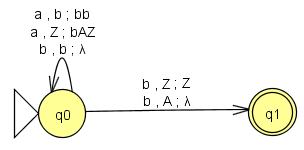
\includegraphics[width=0.5\textwidth]{img/q3/q3.png}
                  \end{figure}

                  \newpage
            \item[4.] [20 Points] For each of the following CFLs, give a "direct" design for an NPDA. That is, it is not acceptable to first find a CFG and then convert it into an NPDA.

                  \textbf{Note:} The start symbol in the stack is $Z$.

                  \begin{enumerate}
                        \item[(a)] $L_1=\{a^nb^{2n+1} : n \geq 0 \}$

                              \begin{figure}[h!]
                                    \centering
                                    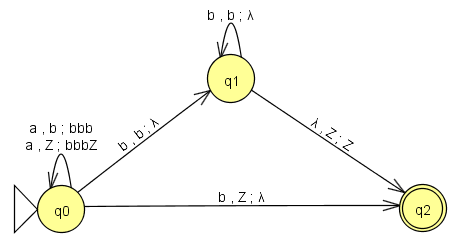
\includegraphics[width=0.6\textwidth]{img/q4/q4a.png}
                              \end{figure}

                        \item[(b)] $L_2=\{w \in \{a,b \}^* : n_a(w) \leq 3n_b(w) \}$

                              \begin{figure}[h!]
                                    \centering
                                    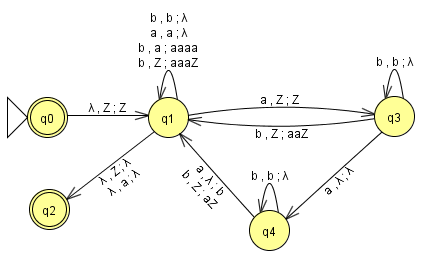
\includegraphics[width=0.7\textwidth]{img/q4/q4b.png}
                              \end{figure}

                  \end{enumerate}
                  \newpage
            \item[5.] [20 Points] Show that the following CFLs are deterministic.
                  \begin{enumerate}
                        \item[(a)] $L_1=\{(ab)^nb(ba)^n : n \geq 0 \} \cup \{(ab)^nb : n \geq 0 \}$

                              \begin{figure}[h!]
                                    \centering
                                    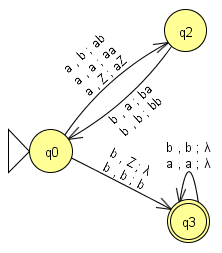
\includegraphics[width=0.4\textwidth]{img/q5/q5a.png}
                              \end{figure}

                        \item[(b)] $L_2=\{w \in \{a,b \}^* : n_a(w) \not= n_b(w) \}$

                              \begin{figure}[h!]
                                    \centering
                                    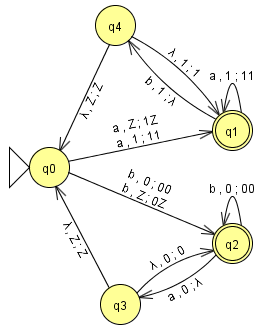
\includegraphics[width=0.5\textwidth]{img/q5/q5b.png}
                              \end{figure}

                  \end{enumerate}

      \end{enumerate}

\end{spacing}

\end{document}